%% This is an example first chapter.  You should put chapter/appendix that you
%% write into a separate file, and add a line \include{yourfilename} to
%% main.tex, where `yourfilename.tex' is the name of the chapter/appendix file.
%% You can process specific files by typing their names in at the 
%% \files=
%% prompt when you run the file main.tex through LaTeX.
\chapter{Introduction}

\section{3D Slicer Interface}
\begin{figure}
	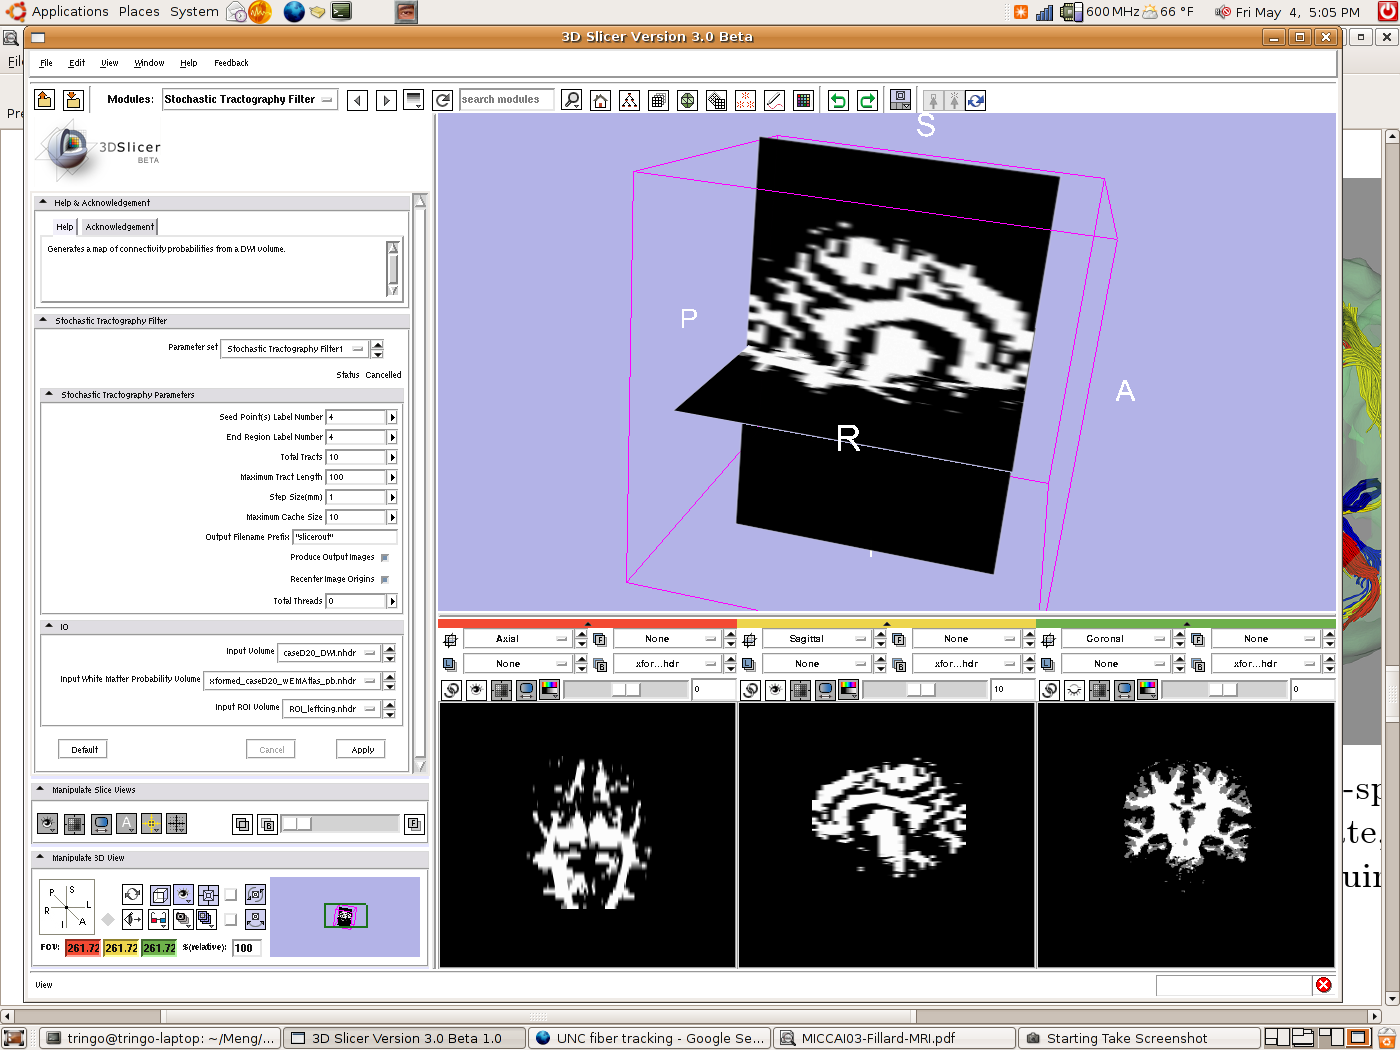
\includegraphics[width=0.5\linewidth]{slicermodule}
	\caption{Stochastic Tractography GUI module within 3D Slicer.}
	\label{fig:Intro}
\end{figure}

Magnetic Resonance Imaging (MRI) is a valuable imaging modality for studying the brain in-vivo.  We can use use MRI to differentiate between tissue types, which is useful in anatomical studies.  Diffusion Weighted Imaging (DWI) and more recently, Diffusion Tensor Imaging (DTI) provides a method to characterize white matter tracts, enabling studies of white matter architecture.

We can visualize DTI data sets using a number of methods.  DTI data sets provide information about the diffusion of water at each voxel, or volume element in the form of diffusion tensors.  A popular technique to visualize these diffusion tensors is to draw fiber tracts which utilize the diffusion information across many voxels.  This technique is known as DTI Tractography.

One possible method to perform tractography is to draw tracts which are oriented with the direction of maximal water diffusion of the voxels they pass through \cite{frimanTMI06}.  However, this method does not provide information about the uncertainty of the generated tracks due to noise or insufficient spatial resolution.  Stochastic white matter tractography addresses this problem by performing tractography under a probabilistic framework.  Stochastic methods provide additional information that enables clinical researchers to perform novel studies.  Several mathematical formulations of probabilistic tractography have existed for some time with the earliest being Behren's implementation\cite{behrensMRM03}.  However, tools which enable widespread adoption of stochastic tractography in clinical studies do not currently exist.  This research implements an easy to use system for performing stochastic white matter tractography based on the algorithm described by Friman et al. \cite{frimanTMI06}.

Researchers have hypothesized that white matter abnormalities may underlie some neurological conditions.  For instance, people characterize schizophrenia by its behavioral symptoms.  A short list of these these symptoms include auditory hallucinations, disordered thinking and delusion \cite{kubickiNYAS05}.  Studies have suggested that these behavioral symptoms have some connection with the neuroanatomical abnormalities observed in schizophrenia patients\cite{kubickiNYAS05}.  Researchers can noninvasively investigate the relationship between brain white matter abnormalities and schizophrenia by using white matter tractography.

Ultimately the success of the system developed in this thesis will depend on its use in the research community.  To this end, we implement the system within the open source ITK Segmentation and Registration Toolkit \cite{itk} framework.  ITK is currently used in many medical data processing applications.  ITK's large existing audience will encourage the system's use in the research community.  Additionally, implementing the stochastic tractography algorithm within ITK facilitates its integration into the 3D Slicer \cite{3Dslicer} for medical data visualization environment.  This thesis implements a 3D Slicer graphical user interface module for the stochastic tractography system, increasing its ease of use and further encouraging its application in clinical research (figure \ref{fig:Intro}).

Finally, we have applied this system towards the analysis of clinical schizophrenia DTI data.  Originally, the data was investigated using non-stochastic tractography methods.  We present a new investigation of the data using the system implemented in this research.  We also compare and contrast the results obtain from stochastic tractography and non-stochastic methods.

In this thesis we shall describe the motivation and implementation of the stochastic tractography system followed by a demonstration of possible applications of the system.  The next chapter  provides a background on nerve fiber tracts, DTI and prior work in white matter tractography.  After the background, the following chapter provides a detailed explanation of the stochastic tractography algorithm.  Then, we will describe the implementation of the algorithm within the ITK framework and optimizations used to improve performance.  Next, we demonstrate the system through an example analysis of frontal lobe nerve fiber bundles.  Finally, we will outline a clinical study which uses the algorithm to investigate differences in frontal lobe nerve fiber bundles in Schizophrenia.
